\graphicspath{{images/program}}

\section{Programm}

% In diesem Kapitel wird das Programm beschrieben, welches die Fotobox steuert.
% Zuerst grober aufbau mitteld diagramm und beschreibung einzelner komponenten.
% Dann in späteren kapiteln genauere beschreibung.

Das gesamte Fotoboxsystem besteht aus mehreren Komponenten, die möglichst nahtlos
miteinander Arbeiten, um dem Benutzer eine einfache und intuitive Bedienung
zu ermöglichen. 

Im Zentrum steht das Windows-Programm, das die Steuerung der Kamera und des
Druckers übernimmt. Es zeigt das Livebild der Kamera auf dem Laptop an,
verarbeitet die aufgenommenen Bilder und sendet sie an den Webserver.

Ein weiterer Bestandteil ist der Webserver. Dieser organisiert die
aufgenommenen Fotos, stellt eine Benutzeroberfläche bereit, über die die Fotobox
konfiguriert werden kann, und ermöglicht den Download der Bilder.

Das Zusammenspiel dieser Komponenten sowie deren genaue Funktionsweise werden
in den folgenden Kapiteln im Detail erläutert.

\newpage

\subsection{Desktop Applikation}

In dem folgenden Kapitel wird die Desktopapplikation 

\begin{figure}[H]
    \centering
    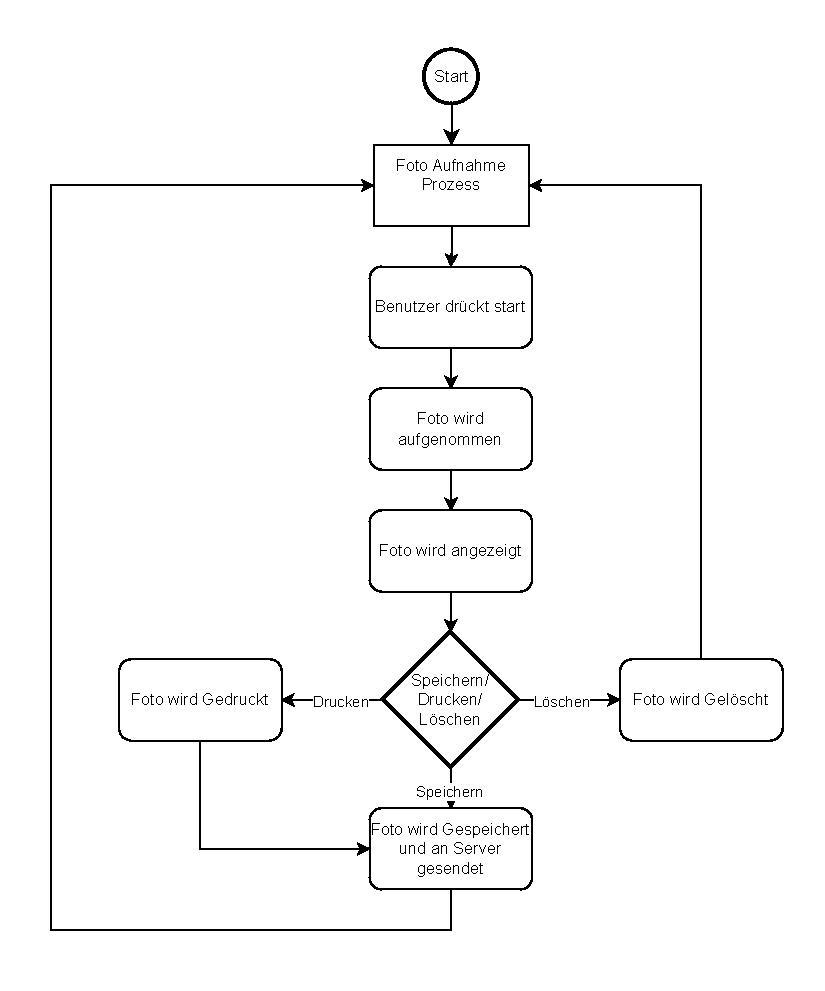
\includegraphics[width=0.75\textwidth]{Ablauf_Foto_Aufnehmen.drawio.pdf}
    \caption{Ablaufdiagramm der Fotoaufnahme.}
    \label{fig:Ablauf_Foto_Aufnehmen}
\end{figure}

In der Abbildung \ref{fig:Ablauf_Foto_Aufnehmen} ist der Ablauf der Fotoaufnahme dargestellt.
Wenn der Benutzer auf den Auslöser drückt, wird ein Foto aufgenommen.
Anschließend wird das Bild auf dem Laptop angezeigt, und der Benutzer hat die Möglichkeit,
auszuwählen, ob das Foto gespeichert, bzw. gedruckt werden soll, oder nicht.